%%%%%%%%%%%%%%%%%%%%%%%%%%%%%%%%%%%%%%%%%
% University/School Laboratory Report
% LaTeX Template
% Version 3.1 (25/3/14)
%
% This template has been downloaded from:
% http://www.LaTeXTemplates.com
%
% Original author:
% Linux and Unix Users Group at Virginia Tech Wiki 
% (https://vtluug.org/wiki/Example_LaTeX_chem_lab_report)
%
% License:
% CC BY-NC-SA 3.0 (http://creativecommons.org/licenses/by-nc-sa/3.0/)
%
%%%%%%%%%%%%%%%%%%%%%%%%%%%%%%%%%%%%%%%%%

%----------------------------------------------------------------------------------------
%	PACKAGES AND DOCUMENT CONFIGURATIONS
%----------------------------------------------------------------------------------------

\documentclass{article}
\usepackage{hyperref}
\usepackage[utf8]{inputenc}
\usepackage[italian]{babel} 
\usepackage[version=3]{mhchem} % Package for chemical equation typesetting
\usepackage{siunitx} % Provides the \SI{}{} and \si{} command for typesetting SI units
\usepackage{graphicx} % Required for the inclusion of images
\usepackage{natbib} % Required to change bibliography style to APA
\usepackage{amsmath} % Required for some math elements 
\usepackage{csvsimple}
\usepackage{adjustbox}
\usepackage{longtable}
\usepackage{booktabs}
\usepackage{color}
\usepackage{listings}
\usepackage{setspace}
\definecolor{Code}{rgb}{0,0,0}
\definecolor{Decorators}{rgb}{0.5,0.5,0.5}
\definecolor{Numbers}{rgb}{0.5,0,0}
\definecolor{MatchingBrackets}{rgb}{0.25,0.5,0.5}
\definecolor{Keywords}{rgb}{0,0,1}
\definecolor{self}{rgb}{0,0,0}
\definecolor{Strings}{rgb}{0,0.63,0}
\definecolor{Comments}{rgb}{0,0.63,1}
\definecolor{Backquotes}{rgb}{0,0,0}
\definecolor{Classname}{rgb}{0,0,0}
\definecolor{FunctionName}{rgb}{0,0,0}
\definecolor{Operators}{rgb}{0,0,0}
\definecolor{Background}{rgb}{0.98,0.98,0.98}
\lstdefinelanguage{Python}{
numbers=left,
numberstyle=\footnotesize,
numbersep=1em,
xleftmargin=1em,
framextopmargin=2em,
framexbottommargin=2em,
showspaces=false,
showtabs=false,
showstringspaces=false,
frame=l,
tabsize=4,
% Basic
basicstyle=\ttfamily\small\setstretch{1},
backgroundcolor=\color{Background},
% Comments
commentstyle=\color{Comments}\slshape,
% Strings
stringstyle=\color{Strings},
morecomment=[s][\color{Strings}]{"""}{"""},
morecomment=[s][\color{Strings}]{'''}{'''},
% keywords
morekeywords={import,from,class,def,for,while,if,is,in,elif,else,not,and,or,print,break,continue,return,True,False,None,access,as,,del,except,exec,finally,global,import,lambda,pass,print,raise,try,assert},
keywordstyle={\color{Keywords}\bfseries},
% additional keywords
morekeywords={[2]@invariant,pylab,numpy,np,scipy},
keywordstyle={[2]\color{Decorators}\slshape},
emph={self},
emphstyle={\color{self}\slshape},
%
}
\setlength\parindent{0pt} % Removes all indentation from paragraphs

\renewcommand{\labelenumi}{\alph{enumi}.} % Make numbering in the enumerate environment by letter rather than number (e.g. section 6)

% CSV import

%\usepackage{times} % Uncomment to use the Times New Roman font

%----------------------------------------------------------------------------------------
%	DOCUMENT INFORMATION
%----------------------------------------------------------------------------------------

\title{Simulazione di un supermercato con Anylogic} % Title

\author{Odore Marco} % Author name

\date{\today} % Date for the report

\begin{document}

\maketitle % Insert the title, author and date

\begin{center}
\begin{tabular}{l l}

Docenti: & Trubian Marco, Malchiodi Dario\\% Instructor/supervisor
Corso: & Simulazione e Teoria delle code
\end{tabular}
\end{center}

% If you wish to include an abstract, uncomment the lines below
% \begin{abstract}
% Abstract text
% \end{abstract}

%----------------------------------------------------------------------------------------
%	SECTION 1
%----------------------------------------------------------------------------------------

\section{Scopo del progetto}

L'obiettivo del progetto è stato quello di simulare, tramite il software Anylogic\footnote{\url{https://www.anylogic.com/}}, diverse dinamiche riguardanti un supermercato, come ad esempio il flusso della clientela, la schedulazione del personale e i diversi servizi che possono essere presenti nell'attività.
\newline
\newline
Il tutto è stato realizzato tramite la versione \emph{learning edition} del software, che presenta alcune limitazioni, come ad esempio il numero massimo di tipologie definibili per gli agenti e un numero massimo per la loro generazione durante l'esecuzione della simulazione\footnote{Durante la simulazione saranno generabili un massimo di 50000 agenti complessivi e in fase di costruzione del modello non è stato possibile definire più di 10 agenti.}.

\section{I servizi}
I servizi simulati nel supermercato sono:
\begin{itemize}
\item Servizio al banco per prodotti di panetteria.
\item Servizio al banco per prodotti di macelleria.
\item Servizio al banco per prodotti di pescheria.
\item Servizio di infopoint.
\item Servizio di pagamento con cassiere.
\item Servizio di pagamento con cassa automatica.
\end{itemize} 

\section{Planimetria supermercato}
Nella figura \ref{planim} è mostrata la planimetria del supermercato e le principali aree di interesse del supermercato:
\newline
\begin{center}

\begin{figure}[h]
\center
\label{planim}
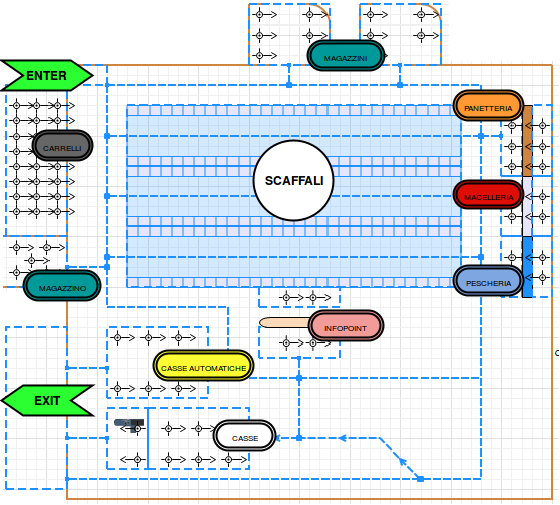
\includegraphics[scale=0.5]{./planimetria1.png}
\caption{Le principali aree di interesse del supermercato.}
\end{figure}

\end{center}



\end{document}